\subsection{Serenity radio system}
As mentioned earlier, Serenity is the spacesuit simulator that the AAs use to conduct analog Mars missions. Its radio system consists of a Motorola Mototrbo SL 2600 handheld radio with a Motorola PMAD4156A antenna, a \emph{push-to-talk} (PTT) button and a Jabra Storm Bluetooth headset. The antenna is attached directly to the handheld radio and the entire system is built into the spacesuit simulator with the upper part of the antenna sticking out. Since the SL 2600 radio supports Bluetooth 4.0, it was decided that communication with the headset should take place via Bluetooth. This has two advantages. Firstly, the AA can put on the headset before donning and thus simply step into the spacesuit simulator, and secondly, the amount of cabling is reduced. The PTT button is wired to the outside of the spacesuit so that the AA can press it to communicate. A schematic structure of this system is illustrated in the figure \ref{fig:tikz_serenity_radio_system}.
\begin{figure}[h!]
	\centering
	

\tikzset{every picture/.style={line width=0.75pt}} %set default line width to 0.75pt        

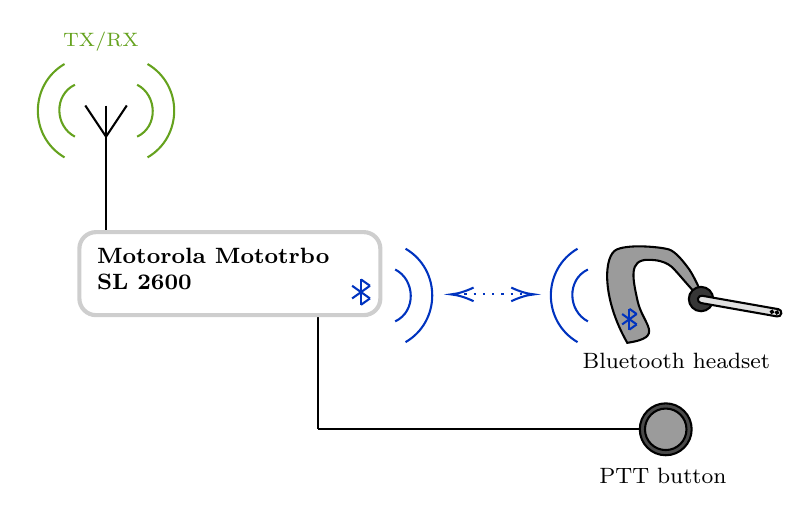
\begin{tikzpicture}[x=0.75pt,y=0.75pt,yscale=-1,xscale=1]
%uncomment if require: \path (0,611); %set diagram left start at 0, and has height of 611

%Straight Lines [id:da6025377414505892] 
\draw    (275,365) -- (275,420) ;
%Straight Lines [id:da8632563010362544] 
\draw    (172.84,264) -- (172.84,324) ;
%Straight Lines [id:da9125480475574657] 
\draw    (162.84,264) -- (172.84,279) ;
%Straight Lines [id:da061481860873287] 
\draw    (172.84,279) -- (182.84,264) ;
%Curve Lines [id:da709923124702297] 
\draw [color={rgb, 255:red, 101; green, 162; blue, 30 }  ,draw opacity=1 ]   (187.84,254) .. controls (197.56,259) and (198.13,274.14) .. (187.84,279) ;
%Curve Lines [id:da449825910233995] 
\draw [color={rgb, 255:red, 101; green, 162; blue, 30 }  ,draw opacity=1 ]   (192.84,244) .. controls (210.09,254.13) and (209.84,279.13) .. (192.84,289) ;

%Curve Lines [id:da6587381411545086] 
\draw [color={rgb, 255:red, 101; green, 162; blue, 30 }  ,draw opacity=1 ]   (157.84,279) .. controls (148.13,274) and (147.56,258.86) .. (157.84,254) ;
%Curve Lines [id:da5450398860583288] 
\draw [color={rgb, 255:red, 101; green, 162; blue, 30 }  ,draw opacity=1 ]   (152.84,289) .. controls (135.59,278.88) and (135.84,253.87) .. (152.84,244) ;

%Rounded Rect [id:dp4917700194036718] 
\draw  [color={rgb, 255:red, 206; green, 206; blue, 206 }  ,draw opacity=1 ][line width=1.5]  (160,333) .. controls (160,328.58) and (163.58,325) .. (168,325) -- (297,325) .. controls (301.42,325) and (305,328.58) .. (305,333) -- (305,357) .. controls (305,361.42) and (301.42,365) .. (297,365) -- (168,365) .. controls (163.58,365) and (160,361.42) .. (160,357) -- cycle ;

%Straight Lines [id:da4309100693896566] 
\draw [color={rgb, 255:red, 0; green, 51; blue, 191 }  ,draw opacity=1 ]   (291.4,350.85) -- (300,356.95) ;
%Straight Lines [id:da87178799188694] 
\draw [color={rgb, 255:red, 0; green, 51; blue, 191 }  ,draw opacity=1 ]   (291.4,356.95) -- (300,350.85) ;
%Straight Lines [id:da19897395538792528] 
\draw [color={rgb, 255:red, 0; green, 51; blue, 191 }  ,draw opacity=1 ]   (295.7,360) -- (295.7,347.8) ;
%Straight Lines [id:da6954421251039244] 
\draw [color={rgb, 255:red, 0; green, 51; blue, 191 }  ,draw opacity=1 ]   (295.7,347.8) -- (300,350.85) ;
%Straight Lines [id:da6576758812784198] 
\draw [color={rgb, 255:red, 0; green, 51; blue, 191 }  ,draw opacity=1 ]   (300,356.95) -- (295.7,360) ;

%Curve Lines [id:da8176024686496981] 
\draw [color={rgb, 255:red, 0; green, 51; blue, 191 }  ,draw opacity=1 ]   (312.16,343) .. controls (321.87,348) and (322.44,363.14) .. (312.16,368) ;
%Curve Lines [id:da5314914665000634] 
\draw [color={rgb, 255:red, 0; green, 51; blue, 191 }  ,draw opacity=1 ]   (317.16,333) .. controls (334.41,343.13) and (334.16,368.13) .. (317.16,378) ;

%Straight Lines [id:da8982122185779959] 
\draw    (275,420) -- (430,420) ;
%Shape: Circle [id:dp17058876030974823] 
\draw  [fill={rgb, 255:red, 74; green, 74; blue, 74 }  ,fill opacity=1 ] (430,420) .. controls (430,413.1) and (435.6,407.5) .. (442.5,407.5) .. controls (449.4,407.5) and (455,413.1) .. (455,420) .. controls (455,426.9) and (449.4,432.5) .. (442.5,432.5) .. controls (435.6,432.5) and (430,426.9) .. (430,420) -- cycle ;
%Shape: Circle [id:dp8498841036551381] 
\draw  [fill={rgb, 255:red, 155; green, 155; blue, 155 }  ,fill opacity=1 ] (432.5,420) .. controls (432.5,414.48) and (436.98,410) .. (442.5,410) .. controls (448.02,410) and (452.5,414.48) .. (452.5,420) .. controls (452.5,425.52) and (448.02,430) .. (442.5,430) .. controls (436.98,430) and (432.5,425.52) .. (432.5,420) -- cycle ;
%Curve Lines [id:da06702286308124483] 
\draw [color={rgb, 255:red, 0; green, 51; blue, 191 }  ,draw opacity=1 ]   (405,368) .. controls (395.29,363) and (394.71,347.86) .. (405,343) ;
%Curve Lines [id:da6829496922473743] 
\draw [color={rgb, 255:red, 0; green, 51; blue, 191 }  ,draw opacity=1 ]   (400,378) .. controls (382.75,367.88) and (383,342.88) .. (400,333) ;

%Curve Lines [id:da5138620347394718] 
\draw [fill={rgb, 255:red, 155; green, 155; blue, 155 }  ,fill opacity=1 ]   (423.98,378.33) .. controls (411.48,356.58) and (412.48,336.08) .. (418.98,333.33) .. controls (425.48,330.58) and (440.82,332.33) .. (443.98,333.33) .. controls (447.14,334.33) and (450.67,338.7) .. (453.5,342.52) .. controls (456.33,346.33) and (462.98,360.59) .. (459.5,357.24) .. controls (456.02,353.89) and (449.86,346.52) .. (447.86,344.33) .. controls (445.86,342.15) and (443.32,338.33) .. (433.98,338.33) .. controls (424.64,338.33) and (426.48,347.08) .. (428.98,358.33) .. controls (431.48,369.58) and (442.48,375.58) .. (423.98,378.33) -- cycle ;
%Shape: Circle [id:dp8048282894012855] 
\draw  [fill={rgb, 255:red, 54; green, 54; blue, 54 }  ,fill opacity=1 ] (453.63,357.24) .. controls (453.63,354) and (456.26,351.37) .. (459.5,351.37) .. controls (462.74,351.37) and (465.38,354) .. (465.38,357.24) .. controls (465.38,360.49) and (462.74,363.12) .. (459.5,363.12) .. controls (456.26,363.12) and (453.63,360.49) .. (453.63,357.24) -- cycle ;
%Rounded Rect [id:dp33219306299895135] 
\draw  [fill={rgb, 255:red, 225; green, 225; blue, 225 }  ,fill opacity=1 ] (458.01,357.1) .. controls (458.18,356.14) and (459.11,355.49) .. (460.07,355.66) -- (496.75,362.12) .. controls (497.72,362.29) and (498.36,363.21) .. (498.19,364.18) -- (498.19,364.18) .. controls (498.02,365.15) and (497.1,365.8) .. (496.13,365.62) -- (459.46,359.16) .. controls (458.49,358.99) and (457.84,358.07) .. (458.01,357.1) -- cycle ;
%Shape: Circle [id:dp48821144483641965] 
\draw   (495.61,363.62) .. controls (495.68,363.35) and (495.95,363.19) .. (496.22,363.26) .. controls (496.49,363.33) and (496.65,363.61) .. (496.58,363.87) .. controls (496.51,364.14) and (496.23,364.3) .. (495.97,364.23) .. controls (495.7,364.16) and (495.54,363.89) .. (495.61,363.62) -- cycle ;
%Shape: Circle [id:dp10261371159326838] 
\draw   (493.19,363.28) .. controls (493.26,363.01) and (493.53,362.85) .. (493.8,362.92) .. controls (494.07,362.99) and (494.23,363.26) .. (494.16,363.53) .. controls (494.09,363.8) and (493.81,363.96) .. (493.55,363.89) .. controls (493.28,363.82) and (493.12,363.54) .. (493.19,363.28) -- cycle ;

%Straight Lines [id:da7564970333053862] 
\draw [color={rgb, 255:red, 0; green, 51; blue, 191 }  ,draw opacity=1 ]   (421.5,364.46) -- (428.5,369.46) ;
%Straight Lines [id:da16147426128772913] 
\draw [color={rgb, 255:red, 0; green, 51; blue, 191 }  ,draw opacity=1 ]   (421.5,369.46) -- (428.5,364.46) ;
%Straight Lines [id:da9003409214844904] 
\draw [color={rgb, 255:red, 0; green, 51; blue, 191 }  ,draw opacity=1 ]   (425,371.96) -- (425,361.96) ;
%Straight Lines [id:da47263261295445824] 
\draw [color={rgb, 255:red, 0; green, 51; blue, 191 }  ,draw opacity=1 ]   (425,361.96) -- (428.5,364.46) ;
%Straight Lines [id:da30877576094905756] 
\draw [color={rgb, 255:red, 0; green, 51; blue, 191 }  ,draw opacity=1 ]   (428.5,369.46) -- (425,371.96) ;

%Straight Lines [id:da6981946954878862] 
\draw [color={rgb, 255:red, 0; green, 51; blue, 191 }  ,draw opacity=1 ] [dash pattern={on 0.84pt off 2.51pt}]  (341,355) -- (377,355) ;
\draw [shift={(379,355)}, rotate = 180] [color={rgb, 255:red, 0; green, 51; blue, 191 }  ,draw opacity=1 ][line width=0.75]    (10.93,-3.29) .. controls (6.95,-1.4) and (3.31,-0.3) .. (0,0) .. controls (3.31,0.3) and (6.95,1.4) .. (10.93,3.29)   ;
\draw [shift={(339,355)}, rotate = 0] [color={rgb, 255:red, 0; green, 51; blue, 191 }  ,draw opacity=1 ][line width=0.75]    (10.93,-3.29) .. controls (6.95,-1.4) and (3.31,-0.3) .. (0,0) .. controls (3.31,0.3) and (6.95,1.4) .. (10.93,3.29)   ;

% Text Node
\draw (167,331) node [anchor=north west][inner sep=0.75pt]  [font=\footnotesize] [align=left] {\textbf{Motorola Mototrbo}\\\textbf{SL 2600}};
% Text Node
\draw (150.69,227) node [anchor=north west][inner sep=0.75pt]  [font=\scriptsize,color={rgb, 255:red, 101; green, 162; blue, 30 }  ,opacity=1 ] [align=left] {TX/RX};
% Text Node
\draw (401,382) node [anchor=north west][inner sep=0.75pt]  [font=\footnotesize] [align=left] {Bluetooth headset};
% Text Node
\draw (409,437) node [anchor=north west][inner sep=0.75pt]  [font=\footnotesize] [align=left] {PTT button};


\end{tikzpicture}

	\caption{Schematic structure of the Serenity radio system.}
	\label{fig:tikz_serenity_radio_system}
\end{figure}

Electrical energy is provided to the SL 2600 via its $2,3\mathrm{Ah}$ lithium-ion battery (Motorola PMNN4468B) which is charged with the electrical energy from the local power grid between missions. At a later point in time, the radio system can be upgraded in such a way, that the SL 2600 can be directly charged from the spacesuit simulator. Similar to the SL 2600, the Bluetooth headset is also supplied with electrical energy from its battery, but can only be charged via the local power grid. 

The maximum transmission power of the SL 2600, as shown in the equation (\ref{eq:power_SER_tx}), is calculated based on its specifications in the table \ref{tab:table_sl2600_specs}.
\begin{table}[h!] % SL2600
	\centering
	\footnotesize
\begin{tabular}{|l|c|}
	\hline
	\multicolumn{2}{|c|}{\textbf{Motorola Mototrbo SL 2600 (VHF digital) specifications}} \\
	\hline
 	Frequency & $136\mathrm{MHz}$ to $174\mathrm{MHz}$ \\
 	Dimensions $\mathrm{(H \times W \times D)}$ & $125,7 \times 55,0 \times 22,7 \mathrm{mm}$ \\%
 	Mass (incl. std. battery) & $190\mathrm{g}$ \\%
	Power supply & $3,7\mathrm{VDC}$ (nominal) \\
 	Average battery life at 5/5/90 duty cycle & $13,5\mathrm{h}$ \\
	Operating temperature & $-30^\circ \mathrm{C}$ to $60^\circ \mathrm{C}$ \\
	Storage temperature & $-40^\circ \mathrm{C}$ to $85^\circ \mathrm{C}$ \\
	RX sensitivity 5\% BER: & $0,25\mathrm{\mu V}$ ($0,19\mathrm{\mu V}$ typical) \\
	TX power output & $0,5\mathrm{W}$ to $3\mathrm{W}$ \\
	Bluetooth version & $4,0$\\
	IP rating & $54$\\
	\hline
\end{tabular}
	\caption{Excerpt from the data sheet of the Motorola Mototrbo SL 2600 handheld radio. \cite{SL2600:2017}}
	\label{tab:table_sl2600_specs}
\end{table}
\begin{equation} \label{eq:power_SER_tx}
	\centering
	P_\mathrm{T,dBW} =  10\mathrm{dBW} \cdot \log_{10} \left( \dfrac{3\mathrm{W}}{1\mathrm{W}} \right) = 4,771\mathrm{dBW}\text{,}
\end{equation}
As with the SLR 1000, the minimum required reception power for the worst case can be taken from the equation (\ref{eq:power_BSt_min}). At this point, the assumption is made that the antenna impedance is $50\Omega$, as no further specifications could be found. It was furthermore assumed that there are no losses in the antenna feed line and that the antenna has a gain of $0\mathrm{dBi}$. 


In cooperation with the Serenity \emph{structures} (STRUC) team, a position for the SL 2600 in the HUT of the spacesuit simulator was found, so that its antenna is upright at a height of $1,65\mathrm{m}$ above the ground for a standard male AA, or at a height of $1,55\mathrm{m}$ above the ground for a standard female AA \cite{Hinker:2007}. Regarding the link budget estimation $h_\mathrm{SER} = 1,55\mathrm{m}$ is used. In its installed position the device can be recharged and, if necessary, removed for maintenance purposes. This fulfills the requirement that the Serenity radio system must fit into the HUT. 

Taking into account the requirements for the operating temperature of the radio system, the data sheets of the SL 2600 (see table \ref{tab:table_sl2600_specs}) and the PTT button, including the wires and connectors involved, show that these are met. Due to the large push area of the PTT button, it was adopted from the Aouda spacesuit simulator, which is the predecessor of Serenity. No specifications were found for the Bluetooth headset and the audio jack that connects the PTT button to the SL 2600. The prototype still needs to be tested in this regard. However, if these do not meet the requirements, a suitable audio jack can be requested directly from Motorola Solutions Inc. and the Motorola EP900w Bluetooth headset can be procured \cite{push_switch:2011, EP900w:2021}.

The most important factor that needed to be considered when developing the radio system was its mass. As stated in the requirements, the combined mass of the W-LAN and VHF based communication systems must not exceed $1000\mathrm{g}$. At the time the Serenity (VHF) radio system was developed, the W-LAN based communication system had a mass of $605,33\mathrm{g}$. The total mass of the (VHF) radio system is $248\mathrm{g}$. This results in a combined mass of $853,33\mathrm{g}$. $9\mathrm{g}$ of this is the mass of the Jabra Storm Bluetooth headset. Should it be replaced by the Motorola EP900w Bluetooth headset, the (VHF) radio system would then have a mass of $261\mathrm{g}$, which results in a combined mass of $866,33\mathrm{g}$. The measurements were conducted with a digital kitchen scale from WMF (Model No.: 06.0873.6040). In the case that the audio jack needs to be changed, its mass is likely to remain the same. Since the W-LAN based communication system is not finished, it cannot be said at this point whether the mass requirement has
 been met. 

